\chapter{Introduction}

\DRG{1}{222} \DRG{3}{112--113}

Figure 1.1 shows the whole territory where Sursilvan is spoken. The Tujetsch valley is located to the west of the territory, whereas the Medel valley is located south-east of the Tujetsch valley.


\begin{figure}
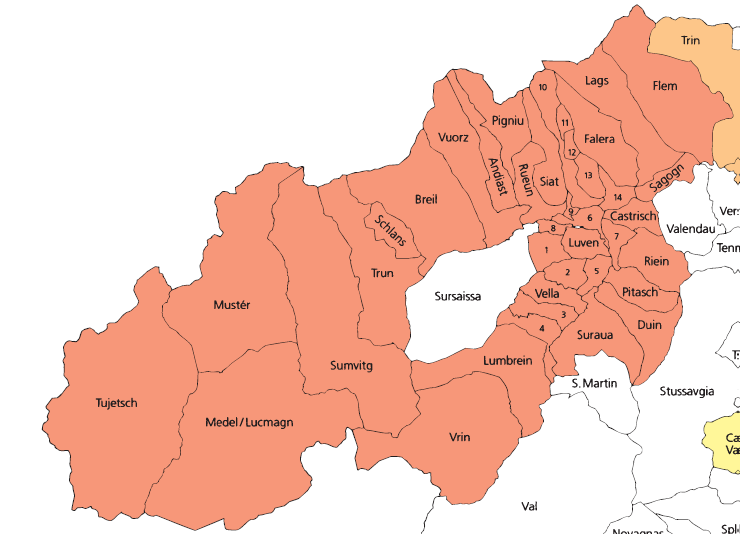
\includegraphics[height=.5\textheight]{figures/Surselva}
\caption{Surselva}

\end{figure}


\section{Previous works}

\citet{Caduff1951}, \citet{Gartner1910}, \citet{Gartner1910}, \citet{Valär2013b}, \citet{Valär2013a},


\section{Corpus}
Documents written in Tuatschin are very scarce. Some sentences and dialogues can be found in the \textit{Dicziunari rumantsch grischun}, in \citet{Büchli1966}, in \citet{Berther1998}, and in. The oral corpus has been established between 2016 and 2018.

The names of the native speakers who participated in our project are made anonymous; their utterances will be labelled with a reference to their sex (m, f), their year of birth and the place where they grew up. These native speakers are listed as follows:


\begin{table}
\caption{List of informants I}
\label{tab:informantsI}
 \begin{tabular}{lllll}
  \lsptoprule
  & f1 & f2 & f3 & f4\\
  \midrule
born & 1923 & 1937 & 1942 & 1947\\
grew up in & Cavòrgia & Sèlva & Sadrún & Ruèras \\
L1 mother & & Tuatschin & Tuatschin & Tuatschin \\
L1 father & & Tuatschin & Tuatschin & Tuatschin \\
%name & Hendry Cec. & Cavegn N. & Levy N. & Giossi L.\\%
 \lspbottomrule
 \end{tabular}
\end{table}

\begin{table}
\caption{List of informants II}
\label{tab:informantsII}
 \begin{tabular}{lllll}
  \lsptoprule
  & f5 & f6 & f7 & f8\\
  \midrule
born &  1961 & 1971 & 1972 &\\
grew up in &  Surajn &  Camischùlas &  Ruèras & Sadrún \\
L1 mother & & Tuatschin & Tuatschin\\
L1 father & & Sursilvan & Tuatschin\\
%name &  Graf B. &  Marino N. & Cathomen N.  & Loretz L.\\%
 \lspbottomrule
 \end{tabular}
\end{table}

\begin{table}
\caption{List of informants III}
\label{tab:informantsIII}
 \begin{tabular}{lllll}
  \lsptoprule
  & m1 & m2 & m3 & m4\\
  \midrule
born & 1935 & 1934 & & 1949 \\
grew up in & Ruèras & Zarcúns & & Sadrún\\
L1 mother & Tuatschin & Tuatschin & & Tuatschin\\
L1 father & Tuatschin & Tuatschin & & Tuatschin\\
%name &  Monn Giu. &  Deflorin Le. & Giossi Vi.  &  Monn Cir. \\%
 \lspbottomrule
 \end{tabular}
\end{table}

\begin{table}
\caption{List of informants IV}
\label{tab:informantsIV}
 \begin{tabular}{lllll}
  \lsptoprule
  & m5 & m6 & m7 & m8\\
  \midrule
born &  & 1951 & 1953 &\\
grew up in &  & Sadrún & Cavòrgja &\\
L1 mother & & Tuatschin \\
L1 father & & Tuatschin \\
%name &  Hendry T. &  Hendry Beni & Hendry W. & Gamboni P. \\%
 \lspbottomrule
 \end{tabular}
\end{table}

\begin{table}
\caption{List of informants V}
\label{tab:informantsIV}
 \begin{tabular}{lllll}
  \lsptoprule
  & m9 & m10 & m11 & m12\\
  \midrule
born &  & 1982 & 1943&\\
grew up in &  &  Sadrún & Ruèras& \\
L1 mother & & & Tuatschin\\
L1 father & & & Tuatschin\\
%name &  Venzin Gi. & Monn Ric. & Brugger Le. & \\%
 \lspbottomrule
 \end{tabular}
\end{table}

\section{Dialectal differences}
There are two main Tuatschin dialects: the dialect of the upper part of the Tujetsch valley, which englobes the villages of Selva and Tschamutt, and the dialect of the lower part of the valley, from Diani to Bugnjaj. These two dialectal areas are divided by a forest, the forest of Sontga Brida (see \citet{Caduff 1952: 3}). The differences are mostly lexical, whereby the forms of the upper dialect correspond to Standard Sursilvan. Some examples are presented in Table xx (see \citet{VicHendry2010: 97}).

\begin{table}
\caption{Differences between the upper and lower dialects}
\label{difdial}
 \begin{tabular}{lllll}
  \lsptoprule
     Lower valley &  Upper valley and Sursilvan & English\\
  \midrule
   \textit{anavaun} & \textit{anavon} & forward \\
   \textit{cuntjants} & \textit{contents} & happy \\
   \textit{tgaglja} & \textit{caglia} & bushes\\
   \textit{ufaun} & \textit{affon} & child \\
\lspbottomrule
 \end{tabular}
\end{table}

Nowadays there are only very few speakers of the upper dialect left.


\section{Glosses}
The glosses used in this grammar are those of the Leipzig Glossing Rules (https://www.eva.mpg.de/lingua/resources/glossing-rules.php), whereby some glosses which are not listed in these rules have been added.

In order to save space, gender and number are only indicated on the first element of the noun phrase, excepted in cases where two or more elements of a noun phrase differ in gender and/or number. Furthermore, indicative mood is not indicated, in contrast to subjunctive, conditional, and imperative mood.





